\section{Adapting online radio channels to their audience} % (fold)
\label{sec:what_i_have_done}

The previous chapter presented poolcasting, an intelligent music selection technique that automatically decides which music to play in contexts where people listen to music in group (discos, parties, radios, bars, offices).
 
This chapter focuses on the domain of online radios, presenting a novel Web radio framework that employs the poolcasting technique to customise radio music channels for their audience.

Most online radios cannot afford expert DJs to programme their channels and are scheduled with random sequences of songs of a given type (e.g., `Rock' songs in a `Rock' music channel).
Employing an intelligent technique like poolcasting can significantly improve the quality of the music in terms of variety, smoothness, customisation and fairness.

Poolcasting Web radio autonomously schedules music channels with good successions of songs and enables listeners to interact among them and with the system in ways that are inconceivable in other Web radios.
To name a few, listeners can:
\begin{itemize}
 \item contribute with new songs to the music broadcast by the radio;
 \item define new radio channels that match their musical tastes; and
 \item evaluate the available songs to influence the music played.
\end{itemize}
%
The breakthrough of Poolcasting Web radio is the creation of a \textbf{social radio} experience.
Listening to radio is normally an individual activity: people ignore who else is listening, cannot interact with each other or control music but for the volume knob.
Most radio stations, both terrestrial and online, are not affected by \emph{who} is actually connected and listeners are forced to waste time in quest of an `ideal' channel.

Poolcasting Web radio takes instead inspiration from digital music services which broadcast music streams that are \emph{personalised} for the audience. 
These services (e.g., Last.fm, Pandora) offer \emph{private} music channels targeted to individuals, while Poolcasting Web radio provides \emph{public} radio channels customised for multiple simultaneous listeners, enabling friends to enjoy music together. % without the need for a DJ. 
Poolcasting Web radio merges the distributed nature of online radios with the personalised nature of music recommenders. 
%Its particular features are detailed hereafter.
%, providing radio channels that everyone can listen to, where the musical content of each channel is customised in real time for the group of listeners.


% 
% \section{Social interaction: active participants}\label{subsection:active}

% subsection passive_listening4 (end)

% section interactive_features_ (end)

\section{Previous work} % (fold)
\label{sec:previous_work9}

Poolcasting Web radio is a user-adaptive system that delivers customised music to a group.
Previous music-related group-adaptive systems are reviewed hereafter, and a characterisation of Internet radios is provided.

\subsection{Group-adaptive systems in music} % (fold)
\label{sub:similar_applications}

A list of previous systems and prototypes designed to adapt music experience to a group of listeners is reviewed hereafter.

\paragraph{MusicFX} % (fold)
\label{par:musicfx_mccarthy98}
\cite{McCarthy98} was a system that automatically selected which radio station to play in a gym according to the taste of the current attendants.
The domain knowledge was made of a set of 91 radio stations categorised by musical style (`Album Rock', `Beach Party', `Flamenco', etc.); user profiles were built by hand, with each member specifying preference for each musical genre; the aggregation was computed using a weighted random selection policy, prohibiting the system from playing any station for which anyone present had a low rating and limiting the period of time that any one genre could play, in order to increase diversity. 
%The main problems of MusicFX are: requires explicit preferences, needs to satisfy one large (possibly heterogeneous) group, individual preferences are not normalised by average user behaviour, and the system has no memory of past user satisfaction, as the authors report:  ``The group preference arbitration algorithm makes its decision based on current information only. I believe that incorporating historical information could improve its decisions''. For instance, the MusicFX system tries to select the right radio station for people working out in a gym at a given time. 
The main lesson learnt from MusicFX was that people had limited desire in compromising their musical preferences with those of some stranger with whom they just happened to work out with.
% paragraph musicfx_mccarthy98 (end)

%\paragraph{hpDJ} % (fold)
%\label{par:hpdj}
%..
% % paragraph hpdj (end)


\paragraph{Smart Radio} % (fold)
\label{par:smart_radio}
\cite{Hayes01b} was a Web-based client-server application to share compilations of music.
%The idea behind Smart Radio is too encourage the sharing of music programmes using automated recommendation techniques
Smart Radio combined automated collaborative filtering and Case-Based Reasoning techniques.
% The differences are: the unit of recommendation is a playlist of 10 music tracks, not a continuous stream of music; only knowledge from the listening history of the participants is considered, no domain knowledge coming from social Web; for the user profile, they only do this: ``By using the most recently played playlist as an indicator of the user's current interests I also solve the practical problem of having to develop a user-profile representation which is compatible with the representation used by the playlists.''; they consider feature such as genres, not genre affinity degrees.
User ratings were gathered combining explicit and implicit feedback. 
Participants could explicitly choose to rate individual tracks or programmes, while the system implicitly gave a positive rating to songs that had been saved to a user's profile and to programmes built from scratch by a user. %Programmes can be put together in a matter of seconds by simple clicking on the desired music item and adding it to the current play list.'' \cite{Hayes01b}.
% paragraph smart_radio (end)


\paragraph{Flytrap} % (fold)
\cite{Crossen02} was an active environment that gathered users' musical tastes and automatically constructed a soundtrack to please everyone in the same room. 
The system combined domain knowledge about how genres of music interrelate and social knowledge about what kinds of transitions between songs people tend to make and broadcast music that satisfied user preferences while fitting its own notion of smoothness.

%Applications: ``Flytrap is an active environment that knows its users' musical tastes and can automatically construct a soundtrack that tries to please everyone in the room. The system works by paying attention to the music that people listen to on their computers. Users of the system have radio frequency ID badges that let the system know when they are nearby. Using the preference information it has gathered from watching its users, and knowledge of how genres of music interrelate, how artists have influenced each other, and what kinds of transitions between songs people tend to make, the ``virtual DJ'' finds a compromise and chooses a song. The system tries to satisfy the tastes of people in the room, but it also makes a play list that fits its own notion of what should come next. Once it has chosen a song, music is automatically broadcast and played.'' \cite{Crossen02} 
\label{par:flytrap}
% paragraph flytrap (end)

\paragraph{The Common Sense Disc Jockey} % (fold)
\label{par:the_common_sense_disc_jockey_ouko02}
\cite{Ouko02} was an application to automatically play music in a dance club environment. 
User profiles were built by a disc jockey observing the audience and completing a form with their age range, ethnic group, geographical provenience, political profile, while a camera tracker estimated the percentage of dancing people.
Preference aggregation was computed following a ``common sense'' rule set; for instance if the crowd appeared to be young Asians, but the exact provenience and profession of the audience were unknown, the system concluded that cross-cultural music from international Pop singers like Britney Spears was best played.
% paragraph the_common_sense_disc_jockey_ouko02 (end)

\paragraph{Jukola} % (fold)
\label{par:jukola}
\cite{OHara04} was an interactive MP3 juke-box that allowed active and collective participation in the choice of music in a public space. 
Jukola allowed people to nominate and vote for songs to get played by means of handheld devices wirelessly connected to a centralised juke-box.
While a song was playing, each device presented four candidate songs to be played next drawn from the list of nominated songs, together with random choices.
Each participant could cast a vote for a candidate and the best ranked song would be played next, according to a plurality voting strategy.
Participants could also upload new songs from their devices to the juke-box to make more music available to the audience.
% paragraph jukola (end)

\paragraph{PublicDJ} % (fold)
\label{par:publicdj_leitich07}
\cite{Leitich07} was a multiplayer game to propose and rate music to listen together with friends.
At each round, users were requested to submit to a server songs they would have liked to hear. 
After analysing the received submissions, the server determined the best matching song with respect to the audience and the last song played. 
Associations between songs were discovered with an acoustic-based approach, combining low-level data (rhythm patterns, statistical spectrum descriptors, rhythm histogram) and high-level data extracted from the files.
The system had no user models and did not keep memory of individual satisfactions.
%The main architectural bottleneck is that songs are submitted and analysed in real time.

%Other approaches have been tried, in form of games, for instance \cite{Leitich07}, a concept for ``music selection in public spaces as multiplayer game ––– PublicDJ, and its prototypical implementation.  The concept is based upon a round based multiplayer game, where each player can submit music tracks to a server. The server analyses submitted tracks and selects the best matching track, based on a former announced criteria for playback.''
% paragraph publicdj_leitich07 (end)

\paragraph{PartyVote} % (fold)
\label{par:party_vote}
\cite{Sprague08} provided groups with a simple democratic mechanism for selecting and playing music at social events.
Aggregated preferences were calculated with a plurality voting approach: songs frequently voted for and popular ones where more likely to be played, whereas boundary voters could listen to at least one song of their choice within two hours from their vote.
% paragraph party_vote (end)

\paragraph{PartyStrands} % (fold)
\label{par:partystrands}
\cite{Strands06} was an interactive system developed by MusicStrands to have bar attendants decide which music would be playing through the night by means of text messages. 
Participants communicated their favourite artists with their mobile phones, and tracks by these artists were played from the venue's loudspeakers (see Fig.~\ref{fig:partystrands}).
The main problem for PartyStrands was a lack of context: every kind of music could be requested, resulting in Heavy Metal tracks immediately followed by Hip Hop tunes or Jazz themes. Moreover, requests came at the cost of a text message, which favoured participants willing to spend more money. 
User requests were simply declined if they could not be satisfied (e.g., when receiving many text messages at the same time) and preferences were aggregated favouring the majority, which often resulted in heavily mainstream musical sequences.
%
\begin{figure}[bthp]
\centering \setlength{\abovecaptionskip}{3pt}
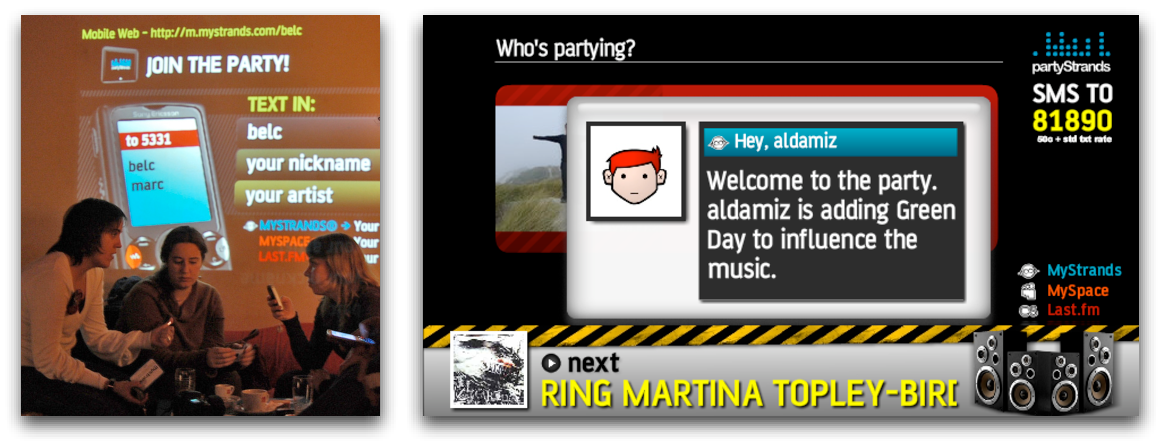
\epsfig{file=img/fig5_1, width=\textwidth}
\caption{PartyStrands in action.}
\label{fig:partystrands}
\end{figure}

% paragraph partystrands (end)

%\paragraph{The Smart Party \cite{Eustice08}} % (fold)
%\label{par:the_smart_party} ``allows user devices to seamlessly and transparently detect, configure, and interact socially in physical locations.'' Does not use domain knowledge, and does not explain how user profiles are created and preferences aggregated.
%% paragraph the_smart_party (end)

%Another similar application is Jukola \cite{OHara04}.

%Another most advanced application is described in \cite{Feldmeier07}, a system consisting of ``wireless sensors that are given to audience members to collect rhythm and activity information from the crowd [...] The pulses received [...] are analysed to detect activity levels and rhythmic features of the audience. These parameters are then available to be mapped to musical content and/or lighting control information. [...] The sound and lighting changes are then realised, to which the audience in turn responds, allowing the experience to build upon itself and giving the users an increased connection to the music.'' DK: Music is generated with loops UP: Nothing, just sensors. AG: what the sensor get (average basically)

%\paragraph{Adaptive Radio} % (fold)
%\label{par:adaptive_radio} uses negative preferences, which makes sense since the system is designed mainly to avoid the playing of music that is disliked by any member (to expand)
%% paragraph adaptive_radio (end)

% subsection similar_applications (end)


\subsection{Internet radios} % (fold)
\label{sub:problems_of_web_radios}

Music is the driving force of the recent transformation of Internet into a social medium. People turn to the Web not just to consume music, but to publish, discuss, share and discover music with friends \cite{McGuire05}.
Indeed social context in music adaptive systems is ``much more important than previously thought'' \cite{McEnnis07}. This preamble explains the success of \textbf{digital music services} such as MySpace, Last.fm and MusicStrands that provide hundreds of millions of users with virtual communities where to interact with other music lovers. % and music streams personalised for each individual.

Given this social demand, it is surprising to observe how online radios offer a service that is very close to old-fashioned AM/FM radios. 
Internet radios first appeared in 1994 \cite{WXYC04} with the intention to broadcast music over the net rather than over the air. 
Millions of online radio stations are available, but the \emph{listening experience} for the audience is still very limited: listeners ignore who else is connected to each station, cannot interact with each other nor request songs or influence the music played.

This has not stopped online radios from growing, with a weekly radio audience estimated in 33 million listeners in the United States \cite{Arbitron08} and a tendency to rise: while listening to AM/FM radio declined four percent, listening to online radio increased 18 percent and free streaming of online music increased 37 percent \cite{NPD05}.

The main competitors for online radios are Web-based music communities that broadcast personalised music streams to their members. 
Last.fm\,---\,the largest of these communities with 37.3 millions monthly unique visitors \cite{Lastfm09}\,---\,offers unlimited personalised channels for a monthly subscription of 3 euros. 

The difference between online radios and digital music services such as Last.fm is that online radios broadcast a fixed amount of music stations that everyone can browse and join at any moment, while in Last.fm channels are private: each members gets a personalised and unique music stream that cannot be shared with other listeners.


% \citet{Mediapost08} also reported that the Internet has surpassed radio as the preferred medium for music among youth in all countries, and that 63 percent of Web radio listeners have a profile on a social Web site, compared to an average of 24 percent.

% Figure~\ref{fig:radio-comparison} shows the main difference between conventional and online radios.
% It can be observed that although Internet radio gains in many aspect, it suffers in the aspect of sociality. 
% 
% \begin{figure}[hbtp]
% \centering \setlength{\abovecaptionskip}{3pt}
% \epsfig{file=img/radio_comparison, width=\textwidth}
% \caption{Comparison of terrestrial and Internet radio.}
% \label{fig:radio-comparison}
% \end{figure}



% section previous_work9 (end)

\section{The Web interface} % (fold)
\label{sec:innovative_features}


The basic service provided by Poolcasting Web radio is online music streaming.
Similarly to other Internet radios, visitors navigate with their Web browsers to the radio home-page (see Fig.\ref{fig:channels-list}), select one channel from the list and start listening to a continuous sequence of songs.
%
\begin{figure}[bthp]
\centering \setlength{\abovecaptionskip}{3pt}
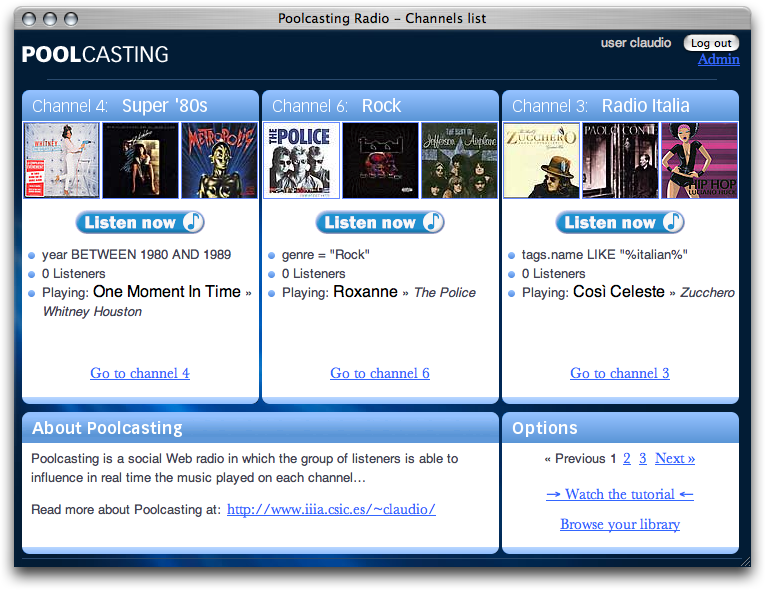
\epsfig{file=img/pwr_list, width=\textwidth}
\caption{Channels list in Poolcasting Web radio home-page.}
\label{fig:channels-list}
\end{figure}

Listening to music is very simple: users just have to click on the `Listen now' button and an appropriate streaming media player (e.g., iTunes, VLC, Winamp) opens up playing the music broadcast from that radio channel.
Another option is to navigate to the Web page of a particular channel (e.g., the `Love the '90s' channel in Fig.~\ref{fig:rock_channel}) and start the integrated Adobe Flash player to listen to music directly in the browser.
%
\begin{figure}[bthp]
\centering \setlength{\abovecaptionskip}{3pt}
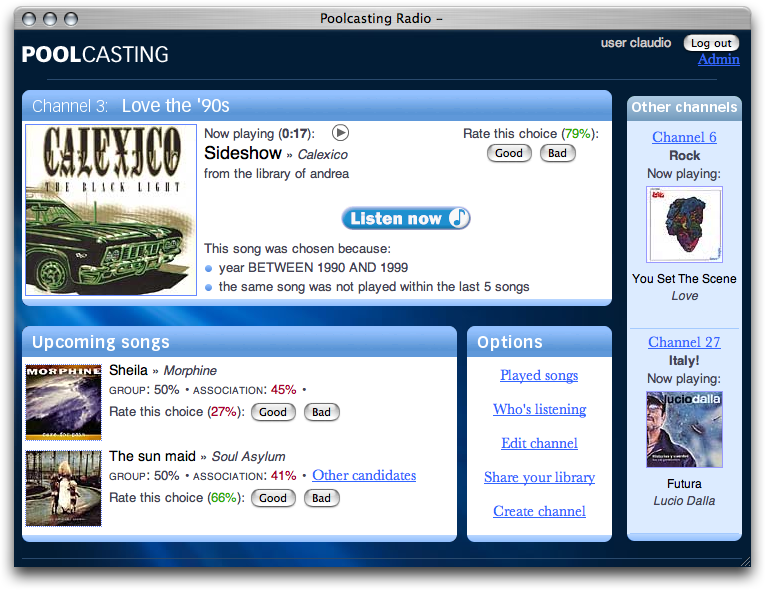
\epsfig{file=img/pwr_channel, width=\textwidth}
\caption{Web interface of a poolcasting radio channel.}
\label{fig:rock_channel}
\end{figure}
%

Tuning into a channel is a concise and intuitive process, so people who just want to passively listen to music can do so.
However, users who want to actively participate in the selection of the music played can do so swiftly as well with the different functions offered by Poolcasting Web radio.

\subsection{Sharing personal music libraries}

Internet radios typically have a large repository of songs stored on a server that some administrators continuously maintain and update to include new releases.
%Still, some listeners may find the library poor or inappropriate; for instance it may contain too many mainstream tracks, or too many obscure songs, or it may be not sufficiently updated.

Poolcasting Web radio abandons this \emph{centralised} storage model in favour of a \emph{distributed} model where the collection of music is provided by the same listeners.
The radio introduces the ability for listeners to share their personal music libraries, that is, to contribute with songs they own to the collection of music the radio can broadcast.

To share their music libraries and become active participants, users click on the `Share your library' link and indicate the path to the local folder where their personal library is stored (see Fig.~\ref{fig:share}). 
This folder has to be accessible from the network via HTTP and the music library managed with Apple iTunes.
%
\begin{figure}[bthp]
\centering \setlength{\abovecaptionskip}{3pt}
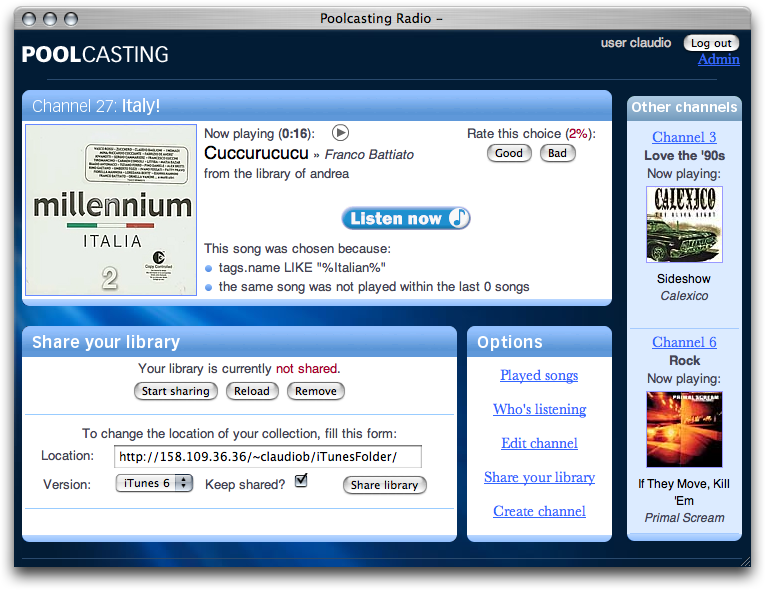
\epsfig{file=img/pwr_share, width=\textwidth}
\caption{Sharing personal music libraries in Poolcasting Web radio.}
\label{fig:share}
\end{figure}
%
After a listener has clicked on `Share library', the system connects to the specified folder and uploads the `iTunes Library.xml' file which contains the list of included songs and listening behaviour data.

Each song in the list is matched against two music recognition Web services.
The first service is OpenStrands, a Web API provided by MusicStrands that returns a unique ID for more than six million songs, fixing wrongly spelled song titles or artist names (e.g., `Obladi Oblada' instead of `Ob-la-di Ob-la-da' or `Mum' instead of `M\'{u}m'). 
Additionally, each song is matched against the Last.fm database through the Last.fm Web API. 
This double check ensures a high identification rate and is also useful to retrieve further information such as the album cover, genre, year and tags of each song.

The `iTunes Library.xml' file also contains the listening habits of each participant; as explained in Sect.~\ref{sec:estimating_individual_preferences} play counts and user ratings are used to automatically infer the preference $i(U,X)$ of each listener for each song.

Each shared library, together with the estimated preferences, is considered by the radio as a new case base.
As described in Sect.~\ref{sec:the_case_based_reasoning_selection_process}, poolcasting holds a collection of case bases, one for each participant;
each case refers to a song, its performing artist and its preference. Figure~\ref{fig:casebases} illustrates with an example how two personal libraries are represented as case bases: songs are matched against OpenStrands Web service, their song and artist IDs are used to univocally identify each song $X$ and artist $a(X)$ while the individual preferences $i(U,X)$ are assessed from the analysis of play counts and user ratings.
%
\begin{figure}[bthp]
\centering \setlength{\abovecaptionskip}{3pt}
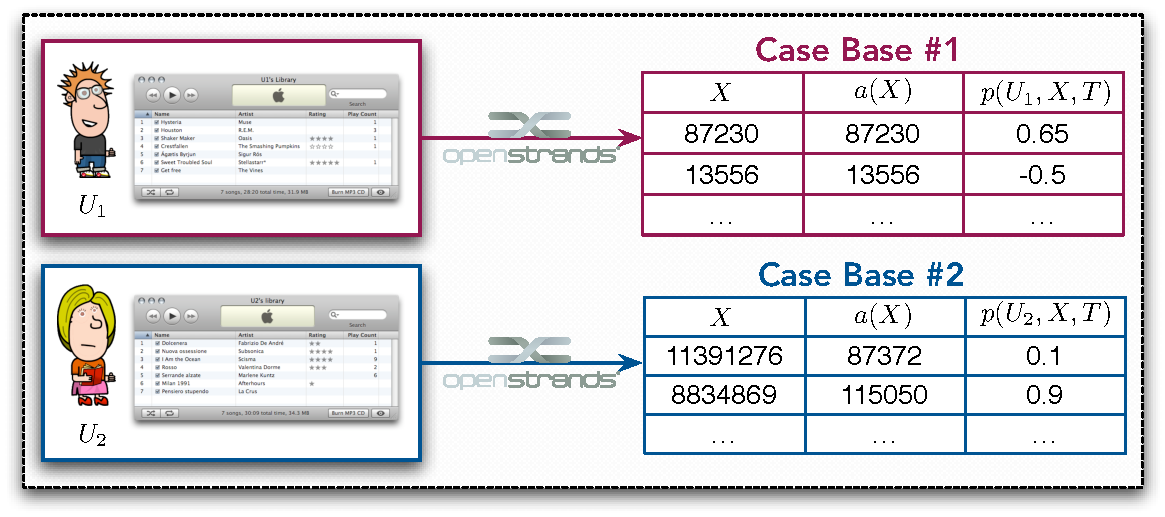
\epsfig{file=img/fig5_5, width=\textwidth}
\caption{From personal libraries to case bases.}
\label{fig:casebases}
\end{figure}

The last piece of information that is collected from the iTunes index file is the location of each song on the hard disk of the library owner.
With this information, the radio can access any shared song as long as the corresponding library owner is connected to the network.

%Having retrieved the index files that describe the content of each shared iTunes library, the system knows the exact location of each song in the hard disk of each participant and, as long as the participants are online, can upload to the radio server any song from any shared library and play them on any radio channel.

% paragraph the_library_parser_ (end)

% The collection of songs shared by all the listeners is called the \textbf{music pool} and will be indicated with $\mathcal{C}$, while the set of all the radio listeners will be indicated with $\mathcal{U}$. Since audience can change over time (people may leave or abandon a channel at every moment), I will also use the notations $\mathcal{C}_T \subseteq \mathcal{C}$ and $\mathcal{U}_T \subseteq \mathcal{U}$ to denote the set of available songs and current listeners of a channel at a given `time' $T \in \mathbb{N}^+$, where time refers to the number of songs played so far in the channel (e.g., $\mathcal{U}_5$ indicates the people listening to the fifth song broadcast on the channel and $\mathcal{C}_5$ indicates the set of songs available to be played at that moment).

The collection of songs shared by all the listeners is called the \textbf{music pool}.
There are several advantages of having a music pool distributed among multiple listeners rather than a centralised radio repository on a server.
Firstly, a distributed collection is more dynamic: when participants share their music libraries, the songs in their hard disks virtually enter the music pool; when one participant leaves, a portion of songs are removed; in general the music pool continuously varies over time.
Next, a distributed collection is more up-to-date: while an administrator would usually update the radio library once a week or a month, individuals add new songs to their libraries every day and these instantly enter the music pool.
A distributed collection also contains more of the longed for `audio not available elsewhere': in fact personal libraries often include songs not publicly distributed (e.g., personal audio material, uncommon records, alternative versions of known themes).
Finally, a distributed collection  contains a finer selection of songs: while a centralised library is normally a massive heterogeneous collection of albums, not filtered by any quality criteria, personal libraries usually contain themes the owner has manually selected and implicitly appreciates.

The fact that the system retrieves and broadcasts music from personal libraries raises questions about copyright issues and licensing policies.
While sharing and streaming music is not an illegal activity per se, most songs are currently published under restrictive licenses that prohibit free public diffusion.
In order to avoid incurring in legal issues, the radio has two options.
The first consists in limiting the service to songs published under non-restrictive licenses such as Creative Commons \cite{CreativeCommons04} that do not forbid sharing or broadcasting.
The second option is to pay the appropriate fee to the national collecting societies in charge of handing out the money to the corresponding music right holders. 
In Spain this monthly fee ranges between 56.26 and 450.11 euros depending on the nature of the service (commercial or not) and on the number of listeners \cite{Sgae06}. %http://www.sgae.es/tipology/est/item/es/1025_291.html]
% when the personal libraries contain DRM-protected songs, these are not broadcast. 

\subsection{Creating radio channels}

Online Web radios typically provide a large but fixed set of channels. Live365, for instance, offers about 6,000 radio stations, ranging from Christmas music to 80's Metal.
Some of these may have no listeners at all; still the administrators will have spent time in their creation and money in songs acquisition, storage space and bandwidth.
Large as the number of channels can be, some listeners may still be unsatisfied for they will not find \emph{the} channel that best fits their taste.

Poolcasting Web radio abandons this authoritarian model and introduces the ability for listeners to create their own channels. 
Participants can browse the list of active channels and, if they do not find the one they like, create a new one by clicking on `Create a channel' (see Fig.~\ref{fig:create}) and indicating its name, description and \textbf{channel pool}, that is, the subset of songs allowed to play. 
The channel pool is defined in terms of genres, tags and years, for instance ``Jazz from 1967'' or ``Italian Electronic Dance''.
Every newly created channel automatically appears in the home-page and is programmed with music that fulfils the specified restrictions.
\begin{figure}[bthp]
\centering \setlength{\abovecaptionskip}{3pt}
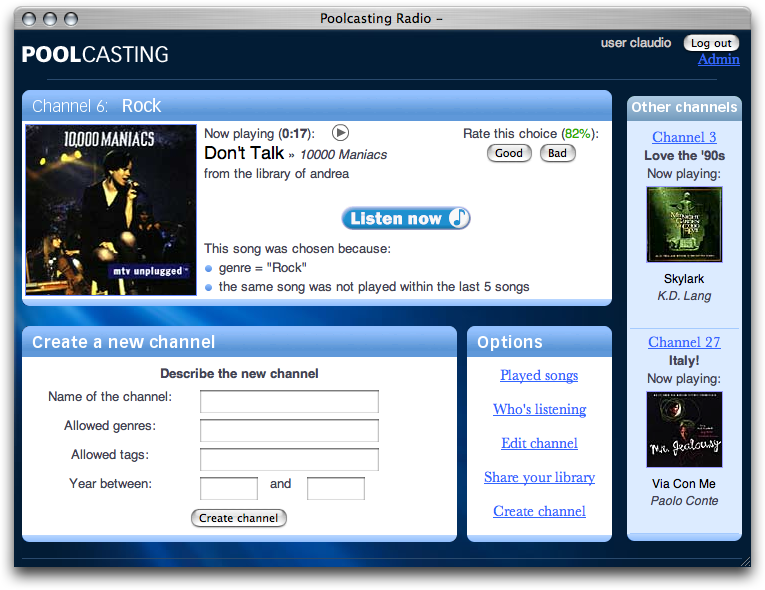
\epsfig{file=img/pwr_create, width=\textwidth}
\caption{Creating radio channels in Poolcasting Web radio.}
\label{fig:create}
\end{figure}

%The music that is allowed to play on each channel depends on two factors: the definition of the channel and the songs that are currently shared on the radio.

%Channels can be defined to play only songs within a particular period, genre or `tag'; for instance a party only plays Dance music or a radio station only plays old Italian themes. The songs that match this filter are called the \textbf{content} of the channel and are indicated with $\mathcal{C}$.


\subsection{Expressing musical preferences} % (fold)
\label{sub:expressing_musical_preferences}

Poolcasting Web radio is similar to common radios in that songs cannot be skipped: they are played from the beginning to the end, one after the other in a continuous stream.
The distinguishing feature is that listeners can express their preferences for every song in the radio and their preferences influence the music scheduled next on each channel.

Listeners can express their musical preferences in two ways. 
The first method is implicit: by sharing one's personal music library.
Shared libraries are viewed by the system as case bases and the individual listening habits data contained (play counts and ratings) are automatically analysed to assess individual preferences $i(U,X)$.

The second method is explicit: providing feedback through the `Good' and `Bad' buttons that appear close to each song (see Fig.~\ref{fig:rock_channel}).
The explicit feedback provided by a participant for a song is indicated by the function $e: \mathcal{U} \times \mathcal{C} \times \mathbb{N}^+ \to [-1,1]$.
The actual value of $e(U,X,T)$ depends on the most recent preference stated through the Web interface at time $T$, as follows:
\begin{itemize}
 \item $e(U,X,T) = 0.5$ if $U$ has clicked once on `Good' for song $X$; 
 \item $e(U,X,T) = 1$ if $U$ has clicked twice or more on `Good' for song $X$; 
 \item $e(U,X,T) = -0.5$ if $U$ has clicked once on `Bad' for song $X$; 
 \item $e(U,X,T) = -1$ if $U$ has clicked twice or more on `Bad' for song $X$; 
 \item $e(U,X,T) = 0$ if $U$ % has not clicked on any button or 
has first clicked on one button and then on the other one for song $X$.
\end{itemize}

% TO ADD: The selection has been limited to two buttons for simplicity!

As defined in \eqref{eq:preference_model2}, the \textbf{individual preference} $p: \mathcal{U} \times \mathcal{C} \times \mathbb{N}^+ \to [-1,1]$ of a person for a song corresponds to the last feedback $e(U,X,T)$ provided, falling back to the preference $i(U,X)$ assessed by the listening habits if no feedback 
was ever provided.
% \begin{equation}
% \label{eq:preference_model}
% p(U,X,T) = 
% \begin{cases}
% i(U,X) & \text{if $e(U,X,T)$ is undefined}\\
% e(U,X,T) & \text{otherwise.}
% \end{cases}
% \end{equation}

% The function $p(U,X,T)$ indicates how much a listener $U$ would like song $X$ to be selected to play next on the channel at time $T$. Calculating this function for all the current listeners with respect to all the songs in the retrieved set brings valuable knowledge about which songs are more or less adapt to satisfy the channel audience.

\subsection{Additional features} % (fold)
\label{sub:additional_features}

Another feature that characterises Poolcasting Web radio is the presence of a live chat integrated in every channel, which makes the members of the audience aware of who else is listening to the same channel (see Fig.~\ref{fig:chat}).
%
\begin{figure}[bthp]
\centering \setlength{\abovecaptionskip}{3pt}
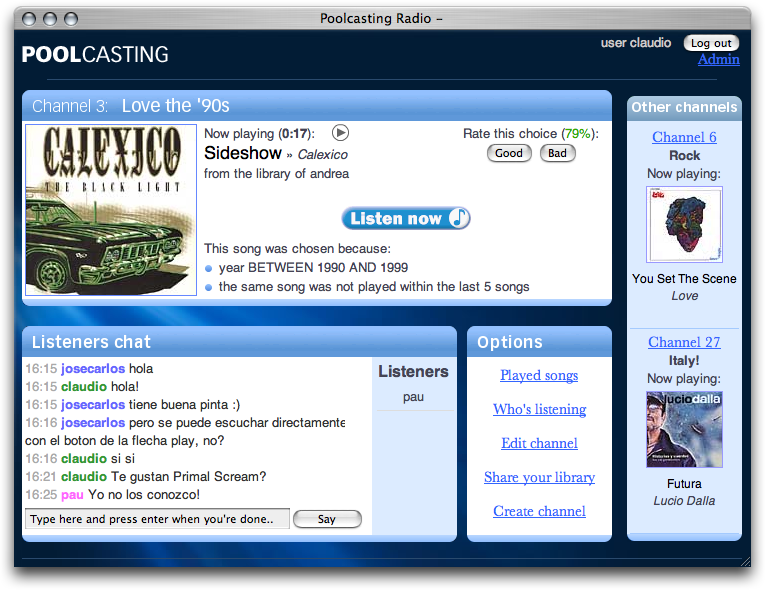
\epsfig{file=img/pwr_chat, width=\textwidth}
\caption{Discussing with other poolcasting listeners.}
\label{fig:chat}
\end{figure}

Poolcasting Web radio also includes an administrative interface that enables a super user to control the various aspects of the radio, from starting and stopping channels to checking the available domain knowledge (musical associations and preferences), from listing the active participants to removing unused channels (see Fig.~\ref{fig:admin}).
%
\begin{figure}[bthp]
\centering \setlength{\abovecaptionskip}{3pt}
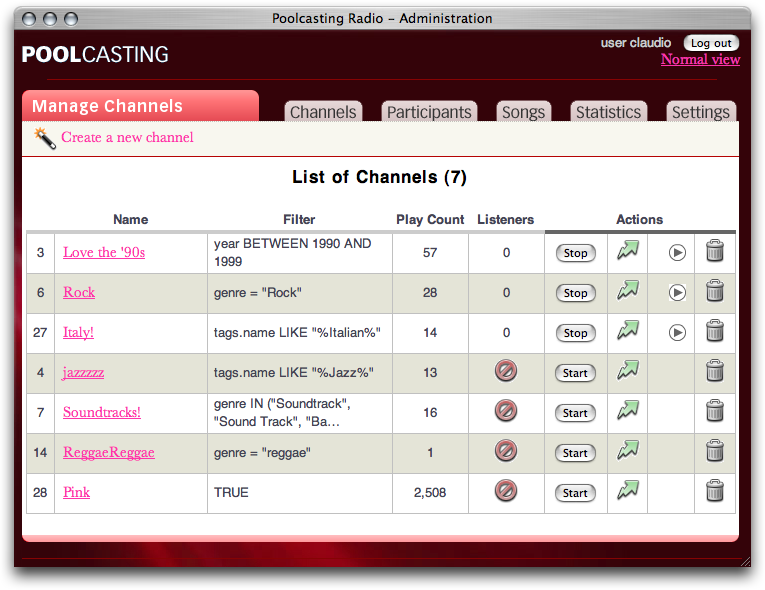
\epsfig{file=img/pwr_admin, width=\textwidth}
\caption{Administration panel of Poolcasting Web radio.}
\label{fig:admin}
\end{figure}

A feature that is common to AM/FM radios but is not present in Poolcasting Web radio is the chance for the audience to directly \emph{request} specific songs.
The reason is that Poolcasting Web radio longs to deliver a musical sequence with a certain musical continuity from song to song (\ref{p:smoothness}).
Accepting direct requests would force the radio to play any kind of music on each channel without guaranteeing smooth transitions from each song to the next.
Direct music requests would also raise issues of fairness in case the system were faced with multiple simultaneous requests and would only be able to please one.
Additionally, online radios that accept requests are regulated by more expensive licensing fees. % collecting societies \cite{Sgae06}.



% subsection additional_features (end)

%Notice that Poolcasting does not immediately and surely play a requested song, for this would infringe most Web radios copyright policies. 
\section{Automated music programming} % (fold)
%\section{The life cycle of a radio channel}
\label{sub:the_reuse_process4}

The music that is played on each channel of the radio is automatically determined by an independent poolcasting CBR process.
The whole radio is initially idle until the first participant joins the system and creates a new channel. At this point, the system spawns a poolcasting process that will determine in real time which songs will be played on that channel.

The songs available to be played are the songs shared by the current participants (music pool), although only a subset % $\mathcal{C}$ 
(channel pool) is allowed to play on each channel (e.g., only `Rock' songs in a channel defined as `genre = Rock').
%
From the channel pool, the system selects at random the first two songs $H_1$ and $H_2$.
The radio connects via HTTP to the personal music libraries where these songs are stored, uploads them to the server and starts broadcasting the first song $H_1$ over the Internet.
Then, the process selects which song $H_3$ to play next; this is accomplished by means of the CBR process introduced in Sect.~\ref{sec:the_case_based_reasoning_selection_process}.

First (retrieve process) the system identifies in the case bases a set of $\kappa = 15$ songs that have not been recently played and that form a smooth musical transition after $H_2$, the previous song in the queue.
These constitute the retrieved set of songs that are good candidates to become $H_3$.

Next (reuse process) the system ranks the candidate set combining the preferences of the listeners with the satisfaction-weighted without misery strategy detailed in Sect.~\ref{sec:social-choice-problem}.
The result is a ranked set where the top ranked candidate is the song that best addresses the goals of customisation and fairness according to the individual preferences stored in the case bases.

The top ranked song is shown in the channel Web page and, if participants do not review their preferences, is played on the channel right after $H_2$.
However at this point (revise process) listeners have the chance to browse the list of candidates and express feedback for each of these songs.

Figure~\ref{fig:pwr_candidates} illustrates the situation of a channel where the first song $H_1$ is playing (`Sideshow' by Calexico), the second song $H_2$ is on the server ready to be played (`Another Invented Disease' by Manic Street Preachers) and `Infidelity (Only You)' (Skunk Anansie) is the best candidate to become $H_3$.
By clicking on `Other candidates', listeners can revise the whole retrieved set and update their preferences for every candidate. 
If a candidate receives a large positive feedback, its group preference degree can surpass that of `Infidelity (Only You)' making that song become the new top ranked candidate.
%
\begin{figure}[tbhp]
\centering \setlength{\abovecaptionskip}{3pt}
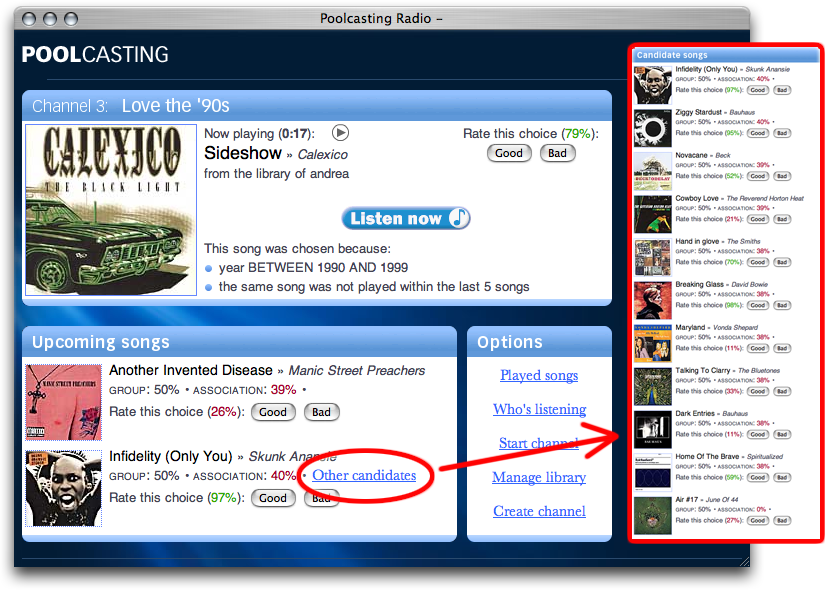
\epsfig{file=img/pwr_candidates, width=\textwidth}
\caption{Retrieved set for a Poolcasting Web radio channel.}
\label{fig:pwr_candidates}
\end{figure}

The revise process continues until the currently playing song $H_1$ terminates. At that moment, the song $H_2$ starts being streamed, the current top ranked candidate is determined as $H_3$ and uploaded to the server to be played next, and the CBR process starts again to select the song $H_4$.

As illustrated in Fig.~\ref{fig:select_and_deliver}, the music played on each channel is therefore automatically selected `one song in advance'.
While the first song $H_1$ is playing, the second song $H_2$ is uploaded to the server and poolcasting determines a set of good candidates to become $H_3$.
The implicit preferences of the audience determine the best ranked song while participants can use the `Good' and `Bad' buttons in the Web interface to revise in real time these preferences.
When $H_1$ ends, song $H_2$ starts, the best candidate to become $H_3$ is uploaded to the server and the process starts again to select $H_4$.
%
\begin{figure}[bthp]
\centering \setlength{\abovecaptionskip}{3pt}
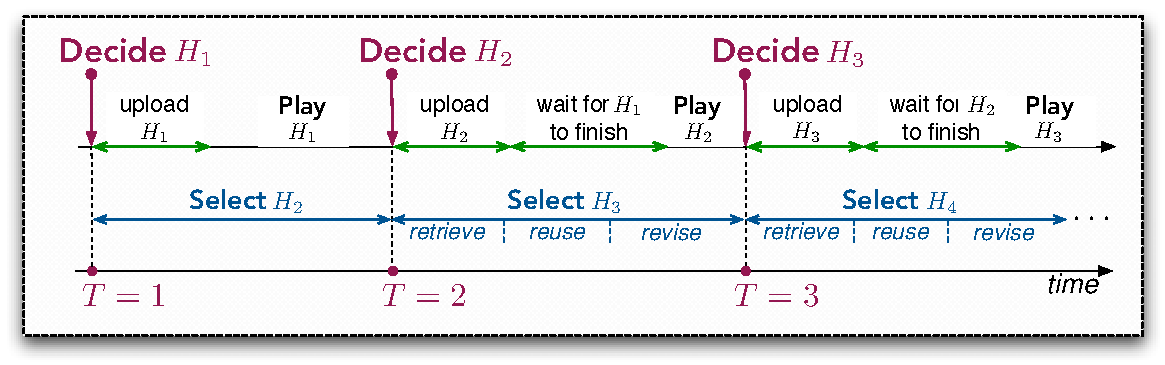
\epsfig{file=img/fig5_10, width=\textwidth}
\caption{A song is playing, the next one uploaded and the next one selected.}
\label{fig:select_and_deliver}
\end{figure}

The reason why poolcasting runs one song in advance is to guarantee an uninterrupted stream of music on each channel.
Whenever a song is playing, the next song has to be already on the server to avoid gaps in the broadcast.
Uploading a song from a personal library and encoding its audio into a proper streaming format require a certain amount of time.
Running the process one song in advance provides the duration of an entire song (typically 3 to 4 minutes) to complete these tasks and also grants enough time to `fall back' to another candidate is the top ranked one suddenly becomes unreachable (e.g., the library where it is contained disconnects from the network).

Music is broadcast from a centralised server rather than from personal libraries in order to guarantee a stable audio quality over time.
If songs were streamed directly from personal libraries (e.g. with a distributed peer-to-peer architecture), the bandwidth of the broadcaster would represent a bottleneck for the audio quality of the stream.
Moreover, if the broadcaster suddenly disconnected from the system, the stream would suffer an undesired break, which is avoided by streaming music from a centralised server after having uploading songs into a temporary buffer.

% ALSO: IF A SONG IS SUDDENLY UNAVAILABLE, THE NEXT IN QUEUE CAN BE LOADED

% The complete CBR process that at every step schedules a new song to play on a channel is illustrated in Fig.~\ref{fig:cbr_process} and is explained hereafter.
% [ NOTE: This figure is wrong: audience goes to pool of songs, and case base also contains preferences, and revise is not clear]
% \begin{figure}[hbtp]
% \centering \setlength{\abovecaptionskip}{3pt}
% \epsfig{file=img/cbr_radio_process, width=\textwidth}
% \caption{The Case-Based Reasoning selection process.}
% \label{fig:cbr_process}
% \end{figure}
% 
% \begin{figure}[hbtp]
% \centering \setlength{\abovecaptionskip}{3pt}
% \epsfig{file=img/iterative_cbr, width=\textwidth}
% \caption{The Case-Based Reasoning selection process.}
% \label{fig:iter_cbr_process}
% \end{figure}
% 
 


% Yet, poolcasting gives the audience the chance to revise their preferences, which can cause the ranking to change.
% As explained in Sect.N, a certain time has to pass from when a song $Z$ is scheduled to when it is actually broadcast. % (namely, the duration of the two  previously scheduled songs $X$ and $Y$). 
% During this time, any listener $P$ can send via the Web interface her explicit preference towards $Z$. If this occurs, the \emph{implicit preference} $g(P,Z)$ that was stored in the Case Base of $P$ (inferred from the music library) is replaced with this new \emph{explicit evaluation} provided.
% For example, if $P$ disapproves of the scheduling of $Z$, then the implicit value of $g(P,Z)$  in the Case Base of $P$ is replaced with the explicit value $-1$.
% Next, since the Case Base has changed, the retrieved set is re-ranked to include this new value in the evaluation of the group preferences.
% This can lead to $Z$ not being the most group-preferred song anymore; in this case, the scheduled song changes to the one that maximises the group preference.
% This process (user evaluations and re-ranking) continues until song $Y$ starts playing on the channel.
% Then, $Z$ is downloaded to the local buffer, and the CBR component restarts, to schedule the next song.
% 
% The generation is assisted so it's not `optimum' but continuous, in real time, and users can `tune' it before it is created (after the ranking).
% 
% 
% The revise process is meant for the audience to update their preferences for the retrieved items.
% If a member expresses a new explicit preference $e(U,X,T)$ for an item, then poolcasting recalculates its group preference.
% This can result in the a different ranking of the retrieved set and in a new item being the candidate with the highest group fairness degree $g(X,T)$.
% 
% When the revise process finishes, poolcasting delivers the best ranked item to the audience, adds it to the list of delivered items as $H_T$ and updates the satisfaction degree $q(U,T)$ of each participant $U \in \mathcal{U}_T$ , so that the least satisfied members will be favoured for the selection of the next items.
% 
% \paragraph{AAAI} % (fold)
% \label{par:aaai6}
% Participants can also use the Web interface to rate whether they liked or not songs they have been listening to on a channel. 
% When a user sends a feedback about a song, her preference model is updated with her new explicit evaluation. 
% For example, if $P$ listens to a new song $Y$ and sends a positive feedback, the system stores the information that $P$ has a high preference for $Y$.
% As a result, the next Reuse processes will be influenced by this new value, and will eventually schedule other songs associated with $Y$ while $P$ is listening. % to that channel.
% % paragraph aaai6 (end)
%
% subsection the_revise_process3 (end)

%Poolcasting Web radio continuously checks \emph{who} is listening to each channel and selects music based on their musical preferences. In this way, listeners do not have to `jump' from one channel to the other looking for music they like. Poolcasting \emph{adapts} the content of each channel for its listeners and not vice versa.


\section{Implementation}\label{subsection:architecture}

%As part of the research, the Poolcasting Web radio architecture described in this chapter has actually been implemented.
%
The development of Poolcasting Web radio took about one year and % and was completed in October 2007. 
its final architecture is illustrated in Fig.~\ref{fig:poolcasting-architecture}.
%
\begin{figure}[bthp]
\centering \setlength{\abovecaptionskip}{3pt}
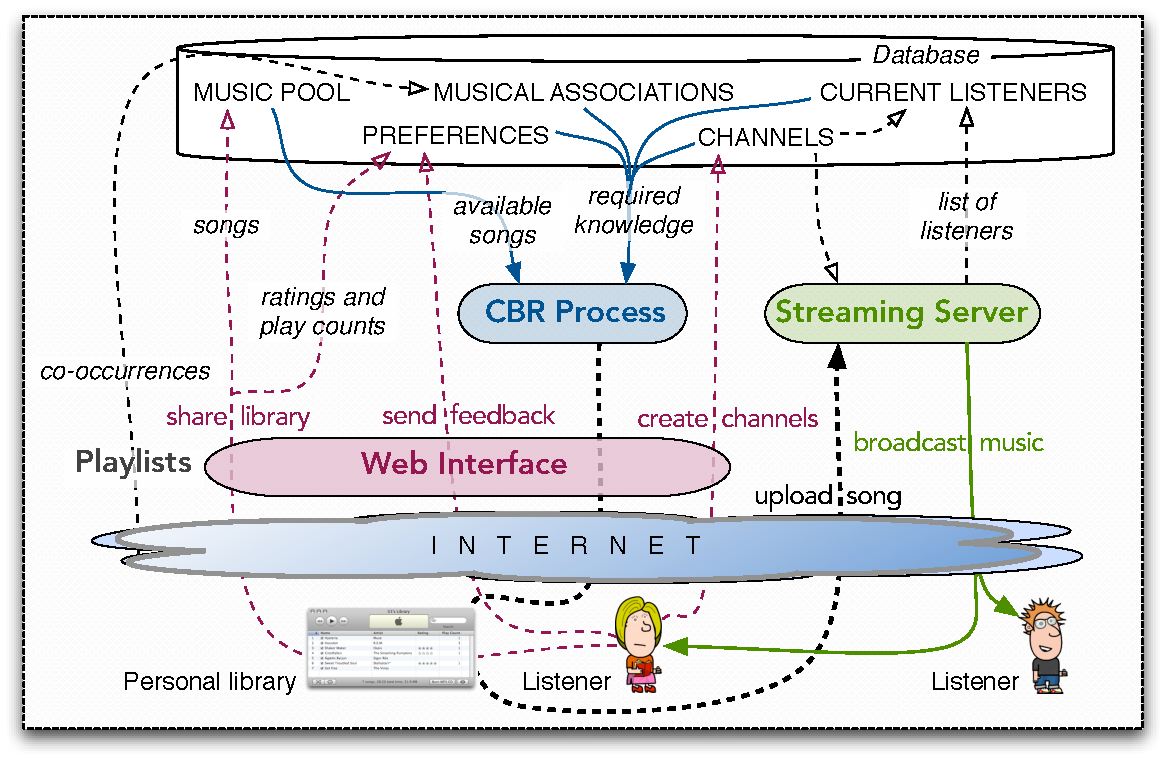
\epsfig{file=img/fig5_11, width=\textwidth}
\caption{Architecture of Poolcasting Web radio.}
\label{fig:poolcasting-architecture}
\end{figure}

The radio is idle until a participant creates a channel through the Web interface.
When this occurs, the streaming server opens a new Internet stream for the channel and a CBR process is started to fill the stream with music.
The CBR process continuously checks in the database which songs are available (music pool), which ones fit the current channel (channel pool), how well each song would go after the last song played (musical associations) and how each of the current listeners like each song (individual preferences).
Having gathered this required knowledge, the process returns the ranked set of candidates that participants can revise by sending `Good'/`Bad' feedback through the Web interface.

When the best candidate is determined, the radio connects via HTTP to the library where the song is contained, uploads the audio file to the server and passes its content to the streaming server as an uncompressed audio signal.
The streaming server encodes the audio into a proper streaming format (either 
MP3 or OggVorbis) that is later broadcast to the connected listeners.

The streaming server also maintains a list of the IP addresses of the listeners of each channel; channels that have not had any listener are automatically disabled after some time, in order to save bandwidth.

The entire framework has been running on a Mac Pro server equipped with two Dual-Core Intel Xeon CPUs at 2.66 GHz and 6 GB of memory. %, providing a private radio service to the IIIA.
%
All the components of the radio have been developed with open source software: \textsf{Ruby on Rails} for the Web interface, \textsf{Apache} for the Web server, \textsf{MySQL} for the database, \textsf{Ruby} for the CBR process, \textsf{liquidsoap} \cite{Baelde08} to manage the music queue and the stream generator, \textsf{icecast} for the streaming server.




% subsection technical_details (end)



% This section works but may be superfluous



\section{Summary} % (fold)
\label{sec:conclusions8}

This chapter has described a new Web radio framework that delivers group-customised music channels, offering an innovative social radio experience.

Poolcasting Web radio combines bottom-up and top-down approaches: users can express their musical preferences while the actual choice of music played is taken by a CBR process that iteratively checks which songs are available and who is listening and selects the songs that most satisfy the current audience.

The advantage of the radio architecture is that user interaction allows the system to model the musical preferences of each listener and exploit them to customise the content of the channels.
Feedback expressed in terms of `Good'/`Bad' preferences offers a direct overview of the listeners' preferences;
in addition, the radio can work without any user interaction by exploiting the implicit knowledge contained in the personal music libraries shared by the participants.

Poolcasting Web radio merges the distributed nature of online radios with the personalised nature of music recommenders, thus offering a groundbreaking Internet service that can satisfy the needs of several Web music listeners.



% section conclusions8 (end)